\chapter{Output Mode Cleaner}
\label{chapter4}
\section{Introduction}
Any optical fields present at the detection photodiodes which do not
produce optical gain will degrade the signal-to-noise ratio of the
readout, by contributing shot noise and technical noise but no signal.

To prevent this SNR degredation, we install an \emph{output mode
  cleaner}, an an optical filter cavity whose resonant mode is matched
to the field of interest.

The light arises from RF sidebands, junk light, and the contrast
defect.  The OMC consists of a Fabry-Perot cavity with length,
g-factor, and finesse chosen to optimally filter the sidebands and
junk light from the desired DARM signal.

The contrast defect is in the same mode as the field we want to keep.

\section{Physical design of the cavity}

The output mode cleaner (OMC) consists of a four-mirror bowtie cavity
with a finesse of approximately 350. The cavity optics and detection
photodiodes are attached to tombstones which are bonded to a glass
slab. This entire optical bench is suspended by a double pendulum,
which in turn rests on an active seismic isolation platform, all of
which is contained within the vacuum envelope. For convenience the
chamber containing the OMC is isolated from the rest of the LIGO vacuum
envelope via a septum window, allowing the independent venting of
this chamber for easier access.

The output of the OMC is split via a 50/50 beamsplitter and directed
onto two high-quantum-efficiency InGaAs photodiodes. The two photodiode
signals allow the formation of sum and difference signals, the difference
providing a diagnostic `nullstream'.

%% Cavity properties [Table]
% These values are all from Sam's document T080144:
% https://dcc.ligo.org/cgi-bin/private/DocDB/ShowDocument?docid=5416
\begin{table}
\centering
\begin{tabular}{l l l l l}
\hline 
parameter          & design      & H1          & L1            & units   \\                    
\hline
perimeter ($p$)    & 1.042       & 1.077       & 1.016         & m       \\
beam waist ($w$)   & 477         & 496         & 463           & \micron \\
Finesse (\Finesse) & 400         & 360         & 360           &         \\
FSR                & 287.7       & 278.3       & 295.2         & MHz     \\  % fsr = c/p
cavity pole        & 360         & 390         & 410           & kHz     \\  % f_c = fsr/(2F)
g-factor           & 0.739       & 0.725       & 0.722         &         \\
HOM freq shift     & 69.4        & 67.2        & 71.8          & MHz     \\
transmission       & 1           & $\geq$0.95  & $\geq$0.90    &         \\
\hline
\end{tabular}
\caption[Output mode cleaner properties (designed and measured)]{Designed and measured properties of the Hanford and Livingston output mode cleaners.}
\label{tab:OMCproperties}
\end{table}

\section{Requirements}

The OMC is required to sufficiently filter the light present at the
output port such that contributions from the RF sidebands and higher-order
spatial modes become negligible. To exclude the RF sidebands, the
cavity length is chosen such that the RF sideband frequencies are
anti-resonant in the cavity, which yields minimum transmission.

\section{Choosing the OMC finesse}

All things being equal, we want the best possible filtering capability
from the OMC.  

The transmission of a lossless critically-coupled cavity is given by
\begin{equation}
T = \frac{1}{1 + \frac{4}{\pi^2}\mathcal{F}^2\sin^2\phi}
\end{equation}
where $\mathcal{F}$ is the cavity finesse and $\phi$ is the cavity's
detuning from resonance.  Since the cavity will be locked to resonance
for the laser carrier, to find the attenuation of other modes, we set
$\phi$ to the detuning of these modes.

The maximum attenuation of a mode is given by $(4/\pi^2)\mathcal{F}^2$.

After filtering by the OMC, we want the shot noise contributions from
unneeded modes to be negligible, and the contribution from noises on
these fields to also be negligible.  Almost any cavity would be
sufficient to reduce excess shot noise contributions.  The need for a
high finesse OMC comes from the need to eliminate audio frequency
noises carried on the RF sidebands and higher-order spatial modes.

\begin{comment}
 h = 6.626068e-34;
 c = 299792458;
 lambda = 1064e-9;
 nu = c / lambda;
 P = 100e-3;
 shotnoise_RIN = sqrt(2*h*nu/P)
\end{comment}

Consider the contribution of intensity noise on the RF sidebands.  Any
residual intensity noise on the RF sidebands will contribute directly
to the DC readout signal.  Assume that the carrier has about 100 mW
power and that the RF sidebands have about the same amount of power,
and assume that the laser intensity noise is $10^{-7}$ RIN.  The shot
noise RIN on 100 mW is (per equation~\ref{eq:shotnoise-asd})
$\sqrt{2h\nu/P} \approx 2\times10^{-9}$.  Thus we need to attenuate
the RF sidebands by at least a factor of 100.

The RF sidebands will not be exactly anti-resonant in the cavity but
will actually lie at about $0.1 fsr$ away from the carrier.  Thus the
attenuation is diminished by approximately $\sin^{-2} (0.1 \pi)
\approx 10$.  So we need attenuation of 1000.  But we really want at
least a factor of 10 margin, so we'll want maximum attenuation of
10000. This means we need a finesse of at least 160.


\section{OMC feedback control systems}

\subsection{Length control (LSC)}

The cavity length must be controlled to maintain the resonance of the
laser carrier.  To sense the mismatch between the laser carrier and
the cavity length, we modulate the cavity length by a small
displacement at high (audio) frequency and monitor the transmitted light
intensity for a signal at the same frequency.  Cavity transmission is
a quadratic function of the frequency/length mismatch; if the
modulation is perfectly symmetric around the point of peak
transmission, there will be no linear coupling.  Effectively, we sense
the first derivative of the transmission with respect to cavity
length.  

\begin{figure}[t]
\centerline{\includegraphics[width=0.5\columnwidth]{figures/ditherdoodle.pdf}
\hfill
\includegraphics[width=0.5\columnwidth]{figures/ditherdoodle.pdf}}
\caption[Cartoon view of dither locking]{\label{fig:dither-doodle}Cartoon view of dither locking}
\end{figure}

\subsubsection{Modeling the dither locking}

Suppose $f(x)$ is a function we wish to maximize; in this case, $f$
gives the power transmitted through the OMC as a function of length
offset.  We let $x = x_0 + A \cos\omega t$, where $A$ is the amplitude
of the dither and $\omega$ is its frequency.  We can expand $f$ as a
power series around $x_0$: 
\begin{align}
f(x) &\approx f(x_0) + f'(x_0)\left(x - x_0\right) + f''(x_0)\left(x-x_0\right)^2 + \cdots \\
     &\approx f(x_0) + f'(x_0)A\cos\omega t        + f''(x_0)A\cos^2\omega t + \cdots
\end{align}
%
The amplitude of the $\cos\omega t$ term is proportional to the first
derivative of $f$ at the current operating point.  (There are also
contributions from higher derivatives, but we assume the lower
derivatives dominate.)

\subsubsection{Noise limits}

Suppose the OMC has coefficient of finesse $F$ and $P$ watts on the
photodiode.  The dither amplitude is $A$ and dither frequency is
$\omega$.  What is the sensing noise limit?

The background is Gaussian white shot noise, equally distributed into
the two demodulation quadratures.  So the noise floor of the
demodulated signal is $(1/\sqrt{2})\sqrt{2 h \nu P}$.

The transmission of the OMC goes like $T(x) = 1/\left(1 + Fx^2\right)$
which has first derivative $T'(x) = 2 F x / \left(1 + F x^2\right)^2 =
- 2 F x + O(x^2)$.  Thus the optical gain is $-2 F A$ watts per meter.

The fast PZT actuator is dithered at 10 kHz and this signal is
synchronously demodulated in the transmitted light.  The bandwidth of
the servo is about 100 Hz.

\section{Input beam alignment control (ASC)}

In addition to controlling the cavity length to keep the carrier
resonant, we must control the pointing of the beam incident on the
OMC.

The decomposition of a given optical field into Hermite-Gauss
eigenmodes is dependent upon a choice of origin and spot size.  The
OMC cavity will select the projection of the incident field onto its
eigenmode.  The optics directing the interferometer output beam to the
OMC

Aligning the input beam to the OMC is a significant problem.  The OMC
can only clean the mode insofar as we can identify the mode we want to
keep.

Several OMC alignment schemes were implemented and utilized.

The simplest alignment control simply uses the two QPDs mounted on the
OMC breadboard.  This has the advantage of being very robust and not
requiring that the OMC already be locked, and so it is ideal for
initial alignment of the OMC before locking the cavity.  The QPD
alignment, however, has no notion of the ideal DC pointing of the beam
and is sensitive not just to the carrier, but also the RF sidebands.

A second alignment scheme is to dither the two steering mirrors each
in pitch and yaw, demodulate the OMC transmitted signal at these
frequencies, and feed back to the mirrors.  This produces an alignment
system which maximizes power transmitted through the OMC.  Because
this is a quadratic point, linear beam jitter coupling is nulled.

Junk light, however, will lead the dither alignment astray.

\begin{figure}
\includegraphics{figures/dithermax.pdf}
\caption[Modal decomposition of a displaced Gaussian]{The sum of a gaussian and a first-order higher order mode
  resembles a displaced gaussian.  A basic dither alignment scheme,
  which maximizes the power transmitted through the OMC, would
  operate near point B, rather than point A.}
\end{figure}

\begin{figure}
\includegraphics{figures/drumhead-dither.pdf}
\caption[Drumhead dither system]{The `Drumhead dither' OMC alignment
  system.}
  
\end{figure}

RF Wavefront sensing.  We did not really consider this.

AF IM WFS.  The same OMC length dither which is used to lock the cavity
length produces an audio-frequency sidebands of the OMC mode in
reflection.  The beats between this light and the light rejected from
the OMC on a pair of photodiodes can be used to produce alignment
error signals.

Beacon dither.  

SNR dither.  Nicolas's scheme.
\subsection{Drumhead dither OMC alignment system}

\begin{enumerate}
\item One of the arm cavity lengths is modulated at high frequency, 9
  kHz.  Intuitively, this modulation `tags' the carrier light emerging
  from the arm.  The modulation is accomplished with a small drive by
  feeding the mechanical drumhead mode of the test mass.
\item The spectral power of the 9 kHz line in the OMC photodiode
  signal is measured by bandpassing the signal around 9 kHz, squaring
  the result, and then low pass filtering.
\item The four degrees of freedom of the two beam steering mirrors are
  modulated (dithered) at a frequency slow compared to the low pass
  filtering in step (2).
\item The measured power in the 9 kHz line is demodulated at the
  steering mirror dither frequencies, producing alignment error
  signals which are fed back to the mirrors.
\end{enumerate}

\subsection{Optimal OMC alignment}

It has been pointed out~\cite{Smith2011Optimal} that even the drumhead
dither alignment scheme is not optimal in the sense of producing the
best shot-noise-limited SNR.

\section{Automatic gain control (UGF servo)}

The optical gain of the interferometer naturally varies slowly as
alignment drifts and the thermal state of the mirrors changes.  The
over-all loop gain must be kept within a few dB of its nominal value
in order for the loop to remain stable.

Before S6 this was done by periodically running a script which
measured the loop gain and adjusted a digital gain to bring it to
nominal.

The flexibility of the realtime code generator allowed us to implement
an automatic gain control servo directly in the OMC front-end.  This
was a nice convenience. 

\section{Residual fluctuations}

\section{Scattering}

The OMC is the largest scattering source in the AS port path.

\subsection{Mode scan}

With the interferometer controlled using the heterodyne readout, the
Output Mode Cleaner can be used as a mode analyzer cavity by varying
the cavity length by at least a free-spectral-range. Because this
range is more than the fast PZT actuator, this is accomplished by
putting a large step into the thermal actuator.
%%  These mode scans can
%% address questions such as:
%% \begin{itemize}
%% \item How well aligned is the OMC?
%% \item How well mode-matched is the OMC?
%% \item How much carrier power is at the output port compared to sideband
%% power?
%% \item How well balanced are the RF sidebands?
%% \item How much junk light is present at the output port?
%% \item Are there any nasty modes near the 00 mode that will sneak through?
%% \item The horizontal/vertical mode separation
%% \end{itemize}
%% The mode scan cannot, by itself, distinguish carrier mode light from
%% the arms vs carrier mode junk light.


\subsection{Scattering}

From the output port, the interferometer appears almost perfectly
reflective.  Any light scattered by the output optics at a small angle
could scatter into the interferometer mode, reflect off of the
interferometer, and interfere with the other fields there.


\section{Interferometer lock acquisition}

Initial lock acquisition of the Enhanced LIGO interferometers is the
same as in Initial LIGO\cite{Evans2002Lock}. Once the interferometer is locked using the
heterodyne readout schemes, the DARM offset is introduced to allow carrier
light to be transmitted to the output port. The Output Mode Cleaner
is then locked to this carrier light. Once the OMC is locked to the
carrier, control of DARM is transferred to the DC readout system.
After this transition, a few other changes are made to engage the
OMC alignment servoes and to put the readout electronics into low
noise mode. At this point the interferometer has reached its operation
configuration and astrophysical data-taking ({}``science mode'')
begins.


\begin{figure}
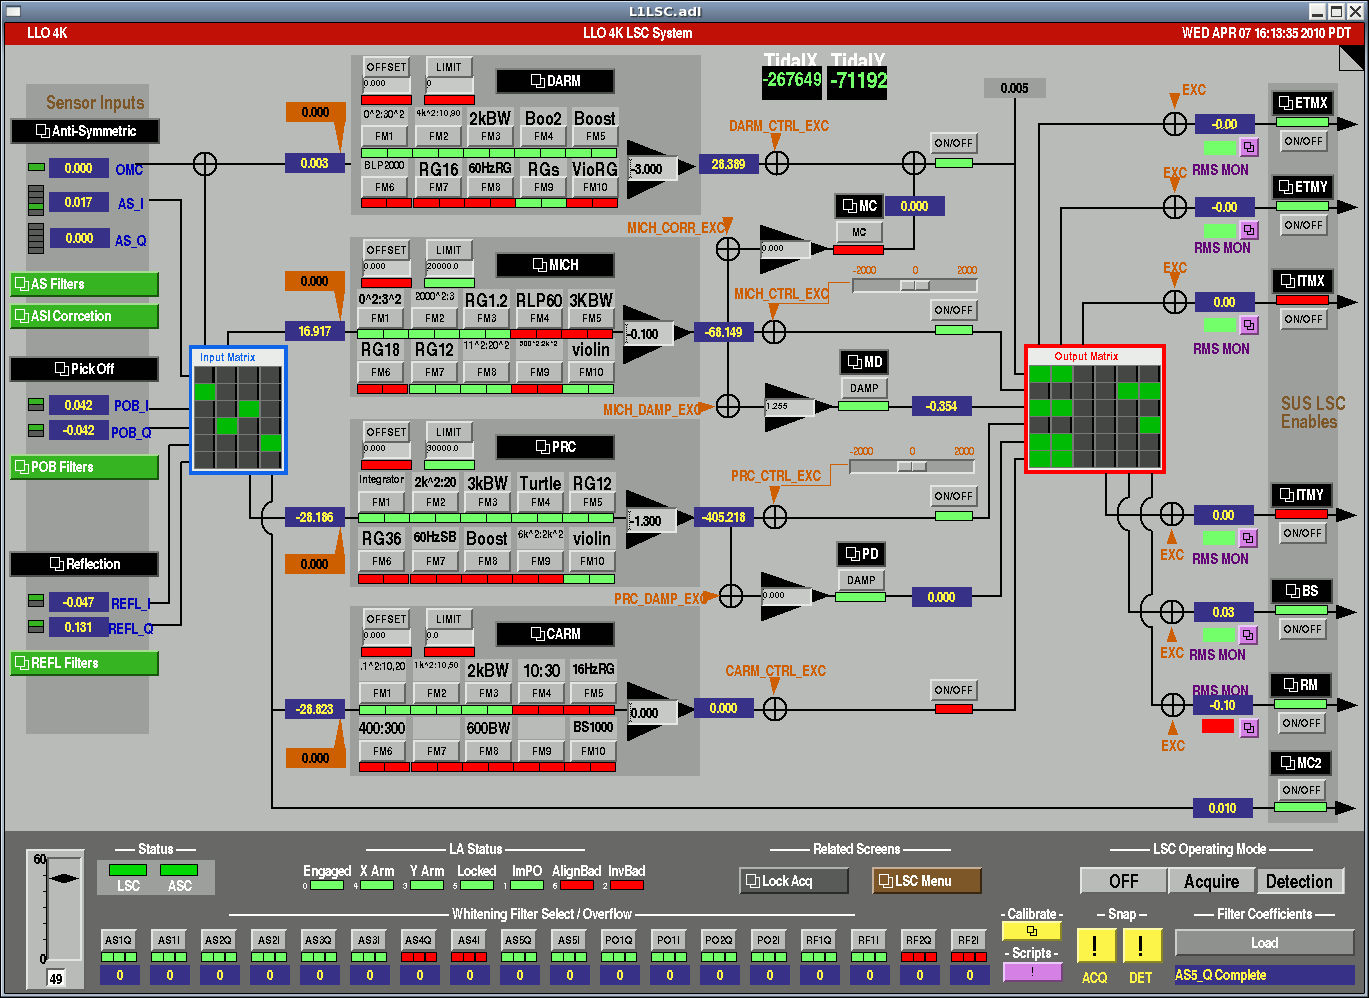
\includegraphics[width=\columnwidth]{figures/L1LSC.png}
\caption[Length Sensing and Control (LSC) control screen]{The control screen for the Length Sensing and Control
  subsystem at Livingston.  The control screen depicts signal flow in
  a generally left-to-right manner.  Photodiodes at the anti-symmetric
  (AS), pick-off (PO), and reflected (REFL) ports are indicated on the
  extreme left.  These signals are combined via an input matrix to
  form the DARM, MICH, PRC, and CARM degrees of freedom.  These
  signals are processed through an array of filter banks defining the
  control filters.  Finally, the signals pass through an output matrix
  and are then directed to the individual optics.}
\end{figure}

\section{Beam diverter}

When the interferometer loses lock, the stored power must be dumped
somewhere. Typically, due to the presence of the power recycling mirror,
the stored power comes out the output port. This high-power transient
is sufficiently strong to burn the detection photodiodes. In order
to prevent this, one of the steering mirrors is used as a fast shutter.
It is able to zero the transmission through the OMC in approx 2 ms.

\section{Observed beam motion}

\section{The Front End}

\begin{quote}
\emph{Be exhorted:} you really can predict the noise floor accurately--to
accept a noisy front end is one of the stupidest and most expensive
mistakes you can make in designing sensitive optical
instruments. Measure it, and make sure you can explain every half
decibel. -- Phil Hobbs, \emph{Building Electro-Optical Systems} \cite{Hobbs2009Building}
\end{quote}

\noindent To achieve the touted SNR improvement of DC readout it is
imperative that the signal not be lost to optical losses, non-optimal
photodiode quantum efficiency, or electronics noise.

\subsection{Photodiodes}
% H1 OMC DC PDs
% https://dcc.ligo.org/DocDB/0005/T0900420/001/T0900420-v1.pdf

Sub-optimal photodiode efficiency counts as a loss just like any other
optical loss. 

The OMC photodiodes are configured in a reverse-biased,
photoconductive arrangement.  An ideal photodiode in such a
configuration will allow one charge carrier to cross the junction for
each incident photon.  The ratio of photocurrent to incident power on
the photodiode is its \emph{responsivity}.  The ratio of a
photodiode's actual responsivity to the ideal is its \emph{quantum
  efficiency}.  At 1064 nm the ideal responsivity is
%
\begin{equation}
\frac{q_e}{h \nu} = \frac{q_e \lambda}{h c} \approx 0.86 \text{ Amps/Watt}
\end{equation}
where $q_e\approx 1.6\times10^{-19}\text{ C}$ is the electron charge.

\begin{comment}
 h = 6.626068e-34;
 c = 299792458;
 lambda = 1064e-9;
 qe = 1.60217646e-19;
 responsivity = qe * lambda / (h * c)
\end{comment}

One lesson (re-)learned during Enhanced LIGO is the need to measure
the characteristics of every individual noise-sensitive component
installed in the final machine rather than relying on measurements of
test samples or typical values.  The photodiodes we originally
installed turned out to have quantum efficiency $\lesssim$ 0.60 while
the test articles of the same part number had quantum efficiency
within a few percent of unity.  Clearly there had been some change in
the manufacturing process that resulted in a greatly diminished
quantum efficiency.  Even for parts which do not show such a dramatic
systematic change, characteristics of individual parts come from some
distribution, and by measuring a batch of parts, the lowest noise
components can be hand picked.

In September 2009 we replaced the bad phototdiodes.  The replacement
photodiodes are Perkin Elmer 3mm InGaAs diodes, part number C30665GH.
The measured quantum efficiency was consistent with unity~\cite{Rollins2009H1}.

\subsection{Electronics}
An optical power of 100 mW on the readout photodiodes will produce a
photocurrent of $i = q_e\lambda/(hc)\cdot 100\text{ mW } = 86\text{ mA}$, which
in turn has a shot noise floor of $\sqrt{2 q_e i}\approx 500 \text{
  pA}/\sqrt{\text{Hz}}$.  Across $100\ \Omega$ transimpedance, this becomes $50
\text{ nV}/\sqrt{\text{Hz}}$.  The noise floor of the readout electronics must
be below this level and not be polluted by any baseband $1/f$ flicker noise.

The main strategy is to aggressively amplify the electronic signal as close to
the photodiodes as possible, so that noises added downstream become
insignificant.  To eliminate even triboelectric effects, the first preamp stages
are placed in-vacuum.  The in-vacuum preamps consist of active filter stages
with two zeros at 8 Hz and two poles at 80 Hz, for a factor of 100 amplification
at 100 Hz.  This is followed by two more pole-zero pairs in satellite amplifiers
on the floor outside the vacuum chamber, for a total gain of 10,000 before the
long run to the racks.

\begin{comment}
h = 6.626068e-34;
c = 299792458;
lambda = 1064e-9;
qe = 1.60217646e-19;
I = qe * lambda / (h * c)
sqrt(2* qe * I)
\end{comment}

\begin{figure}
\includegraphics[width=\columnwidth]{figures/D0901817.pdf}
\caption[Output Mode Cleaner photograph]{Photograph of the Output Mode
  Cleaner used at Livingston, taken \emph{ex situ}.  Photometry by Sam
  Waldman.  This diagram has document number \href{https://dcc.ligo.org/cgi-bin/private/DocDB/ShowDocument?docid=4713}{D0901817}.  Only one of
  the two DC photodiodes is installed in this photo.}
\end{figure}
% Hanford: 
% https://dcc.ligo.org/cgi-bin/private/DocDB/ShowDocument?docid=4714

Additional references: \cite{Prijatelj2010,Bork2009ELIGO,Betzwieser2004Study}
